Rigorous free-energy calculations using molecular dynamics (MD) simulations have become an important tool to estimate binding free energies of novel compounds for lead optimization in drug discovery \cite{Cournia2017, Armacost2020,Cournia2020}. Although computationally relatively expensive, these methods are needed to properly account for entropic contributions introduced by protein/ligand conformational changes, entropy-enthalpy compensation, and the desolvation of a ligand \cite{Chodera2013}.

Computational free energy calculations typically make use of thermodynamic cycles, i.e., the transitive difference relations of idealized states of the system of interest that are representable by a graph. For instance, to estimate the binding free energy of five compounds, a ``state graph'' can be constructed (Figure~\ref{fig: StateGraph}), where the nodes represent the end states and the edges the free-energy differences between them. Although not impossible \cite{Aldeghi2016}, the direct calculation of (absolute) binding free-energies ($\Delta G^\text{bind}_i$) is generally very challenging to achieve computationally \cite{Cournia2017}. A simpler alternative is to calculate the alchemical free-energy differences between two compounds $i$ and $j$ in a given environment ($\Delta G_{ji}^{env}$) and then compare the relative binding free energy $\Delta \Delta G^\text{bind}_{ji}$ with the difference of the $\Delta G^\text{bind}_i$ obtained from experiments \cite{Jorgensen1988, Merz1991},
\begin{equation}
    \Delta \Delta G^\text{bind}_{ji} = \Delta G_{ji}^{\text{protein}} - \Delta G_{ji}^{\text{water}}
    = \Delta G^\text{bind}_j - \Delta G^\text{bind}_i
\end{equation}

Conventional free-energy methods such as thermodynamic integration (TI) \cite{Kirkwood1935} and free-energy perturbation (FEP) \cite{Zwanzig1954} introduce a coupling parameter $\lambda$ to define a pathway from end state $i$ ($\lambda=0$) to end state $j$ ($\lambda=1$). In practice, simulations at discrete intermediate $\lambda$-points are performed to obtain converged free-energy differences.

%
If a (large) series of $N$ compounds is investigated, the free-energy difference for all $(N(N-1))/2$ pairs of ligands would in principle have to be calculated. To reduce the computational cost, automatic schemes have been developed to identify the edges in the state graph (Figure \ref{fig: StateGraph}) with the smallest perturbations such that all nodes (for a given environment) are connected \cite{liu2013,wang2015,yang2020}. It is thereby important to include some cycles as cycle closure is a frequently used measure to assess convergence. 
Nevertheless, manual optimizations may sometimes be required to determine the best sampling strategy \cite{Jespers2019}.
Furthermore, calculating only a subset of the edges leads to a larger uncertainty in the estimated free-energy difference for pairs that are no longer directly connected. As $\Delta \Delta G^\text{bind}_{ji}$ values are often relatively small, the increased uncertainty may negatively impact the usefulness of such calculations in practical applications. 

\begin{figure}[h]
    \centering
    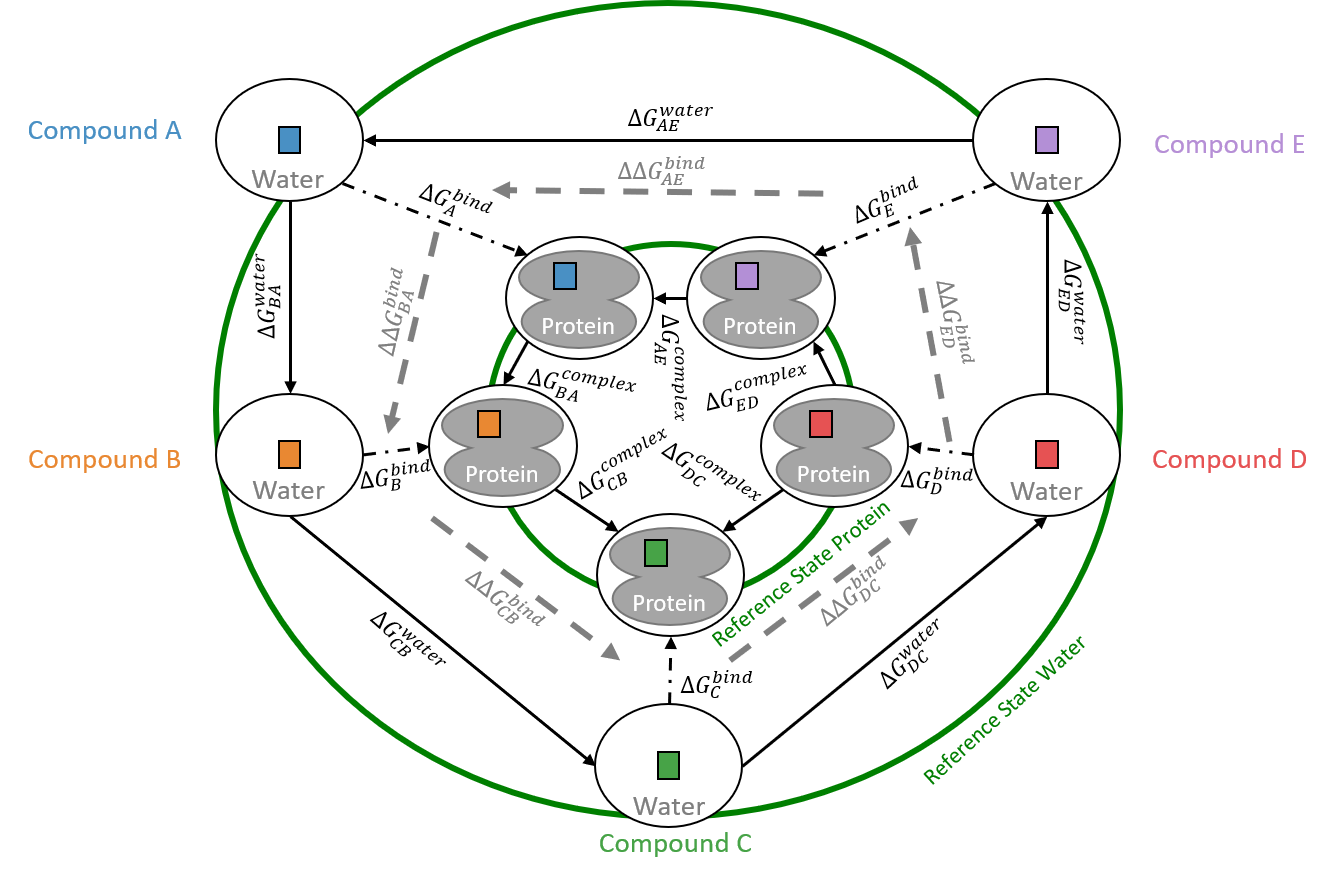
\includegraphics[width=\columnwidth]{fig/intro/State_graph.png}
    \caption{State graph to calculate relative binding free energies, where the nodes represent specific compounds $A$ - $E$ in a particular environment (water/protein). 
    The connecting (directed) edges describe the transformations from one end state to another. The dashed-dotted arrows denote the direct calculation of the (absolute) binding free energy of compound $i$ to the protein, $\Delta G_{i}^\text{bind}$, whereas solid arrows indicate alchemical transformations between compound $i$ to compound $j$ in a given environment. From the resulting $\Delta G_{ji}^\text{env}$, $\Delta \Delta G^\text{bind}_{ji}$ can be calculated and compared with the value obtained from the difference of the experimentally determined $\Delta G_{i}^\text{bind}$ (gray dashed arrows).
    In pathway-dependent methods, each edge between two end states is calculated separately. With (RE-)EDS, all end states in a given environment can be considered simultaneously in a single simulation of a reference state (green circles).}
    \label{fig: StateGraph}
\end{figure}

%The advantage of pathlessness
An attractive and more efficient alternative to path-dependent methods is to simulate a reference state, which includes all $N$ end states simultaneously, without the specification of pathways (green rings in Figure \ref{fig: StateGraph}). Such a reference state is provided by the enveloping distribution sampling (EDS) \cite{Christ2007, Christ2008, Christ2009a, riniker2011} method. The EDS reference state can be further tuned for optimal sampling with parameters. Note that cycle closure is guaranteed by definition in this approach.
%
In order to enhance sampling further, combinations of EDS with enhanced sampling methods were developed such as replica-exchange EDS (RE-EDS) \cite{Lee2014, Sidler2016, Sidler2017} and accelerated EDS \cite{Perthold2018, Perthold2020}.

%conclusion:
In this study, we present an improved automated workflow for RE-EDS simulations that was restructured into two phases. The first phase aims to automatically estimate method parameters that otherwise had to be provided by the user. The second phase automatically optimizes the estimates from the first phase to retrieve a robust parameter set. The final production phase calculates the relative binding free energies of multiple ligands from a single simulation per environment. 
The robustness and versatility of the RE-EDS workflow are demonstrated on a series of five inhibitors of human checkpoint kinase 1 (CHK1) \cite{Huang2012}.
These ligands were selected by Wang \textit{et al.} \cite{Wang2017} as a challenging benchmarking set for FEP calculations since the changes between these ligands exemplify different types of core-hopping transformations (i.e. ring size change, ring opening/closing, and ring extension). Special soft bond-stretching terms were developed to be able to handle these transformations \cite{Wang2017}. In contrast to many other methods, no such special soft bonds are required with RE-EDS as we can use a ``dual topology'' approach \cite{Riniker2011} in a straightforward manner. 
